\chapter{Enabling technologies} \label{2cap:design}
%
%\label{}

\section{Hardware}

\subsection{PLC SIMATIC S7-1200}
The PLC SIMATIC S7-1200 with CPU 1215C AC/DC/RLY (Figure\ref{fig:plc}) is a PLC produced by Siemens and it was used in this project in order to realize the sequence control of the robotic arm. \newline
It is characterized by:
\begin{itemize}
    \item 14 24V digital inputs;
    \item 10 relay outputs;
    \item 2 analog inputs;
    \item 2 analog outputs.
\end{itemize} 

\begin{figure}[!h]
\begin{center}
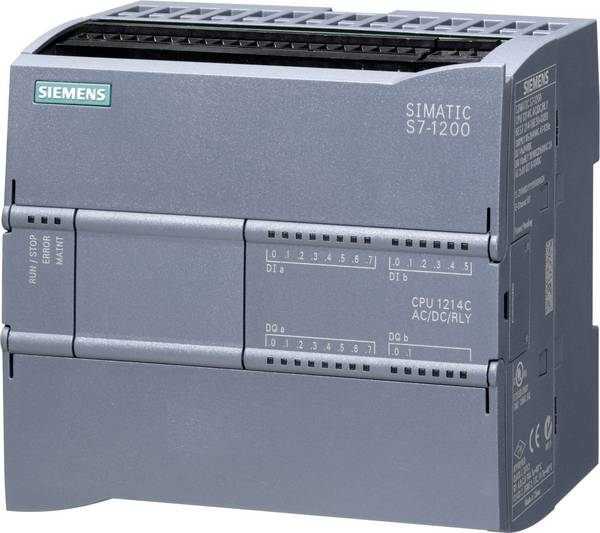
\includegraphics[width=0.4\linewidth]{capitolo2/figure/plc.jpeg}
\caption{Siemens SIMATIC S7-1200 1215C AC/DC/RLY PLC}
\label{fig:plc}
\end{center}
\end{figure}

\subsection{Fischertechnik 3D-Robot 24V}

The 3D-Robot 24V (Figure\ref{fig:robot}) is a robotic arm produced by Fischertechnik. It is a 3-DOF (3 degrees of freedom) robot and in particular it is composed by:
\begin{itemize}
    \item a revolute joint;
    \item 2 prismatic joints (up/down and frontward/backward);
    \item a gripper as end-effector.
\end{itemize}

\begin{figure}[!h]
\begin{center}
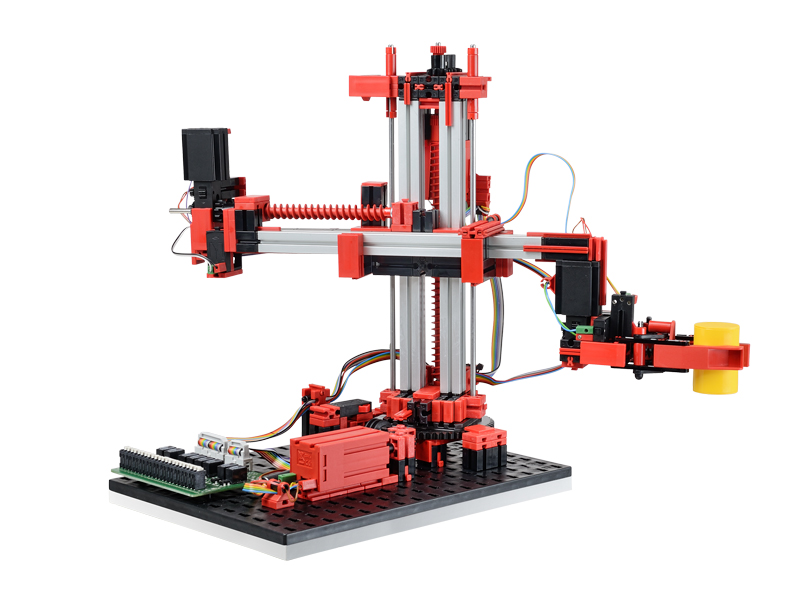
\includegraphics[width=0.8\linewidth]{capitolo2/figure/3D-Robot-24V.jpeg}
\caption{Fischertechnik 3D-Robot 24V}
\label{fig:robot}
\end{center}
\end{figure}
Thus the robot is characterized by a cylindrical geometry: its workspace is a portion of a hollow cylinder.

\subsubsection{Mini switches}
The robot has four mini switches (Figure\ref{fig:switch}) that are pressed respectively in four different conditions:
\begin{itemize}
    \item the gripper is fully open;
    \item the end-effector is completely brought back;
    \item the horizontal arm is completely brought up;
    \item the robot is completely rotated clockwise.
\end{itemize}

\begin{figure}[!h]
\begin{center}
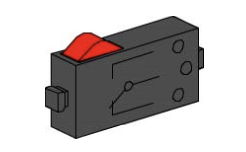
\includegraphics[width=0.4\linewidth]{capitolo2/figure/mini_switch.png}
\caption{Mini switch}
\label{fig:switch}
\end{center}
\end{figure}

\subsubsection{Pulse counters}
The robot has two pulse counters, that can be used to understand respectively:
\begin{itemize}
    \item how much the gripper is open;
    \item how much the horizontal arm is moved frontward.
\end{itemize}

In fact, the pulse counters are switches that are automatically pressed each time a gear involved in the corresponding movement rotate of a certain angle, producing a certain quantity of movement.

\subsubsection{Encoders}
The robot has two motor encoders (Figure\ref{fig:encoder}) with a maximum frequency of 1 KHz, that can be used to understand respectively:
\begin{itemize}
    \item how much end horizontal arm is moved down;
    \item how much the robot is rotated.
\end{itemize}

\begin{figure}[!h]
\begin{center}
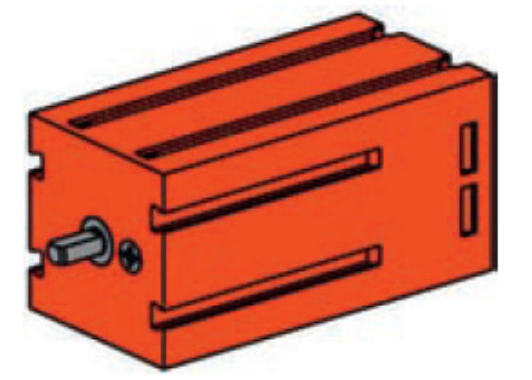
\includegraphics[width=0.4\linewidth]{capitolo2/figure/encoder.png}
\caption{Motor encoder}
\label{fig:encoder}
\end{center}
\end{figure}

\begin{figure}[!h]
\begin{center}
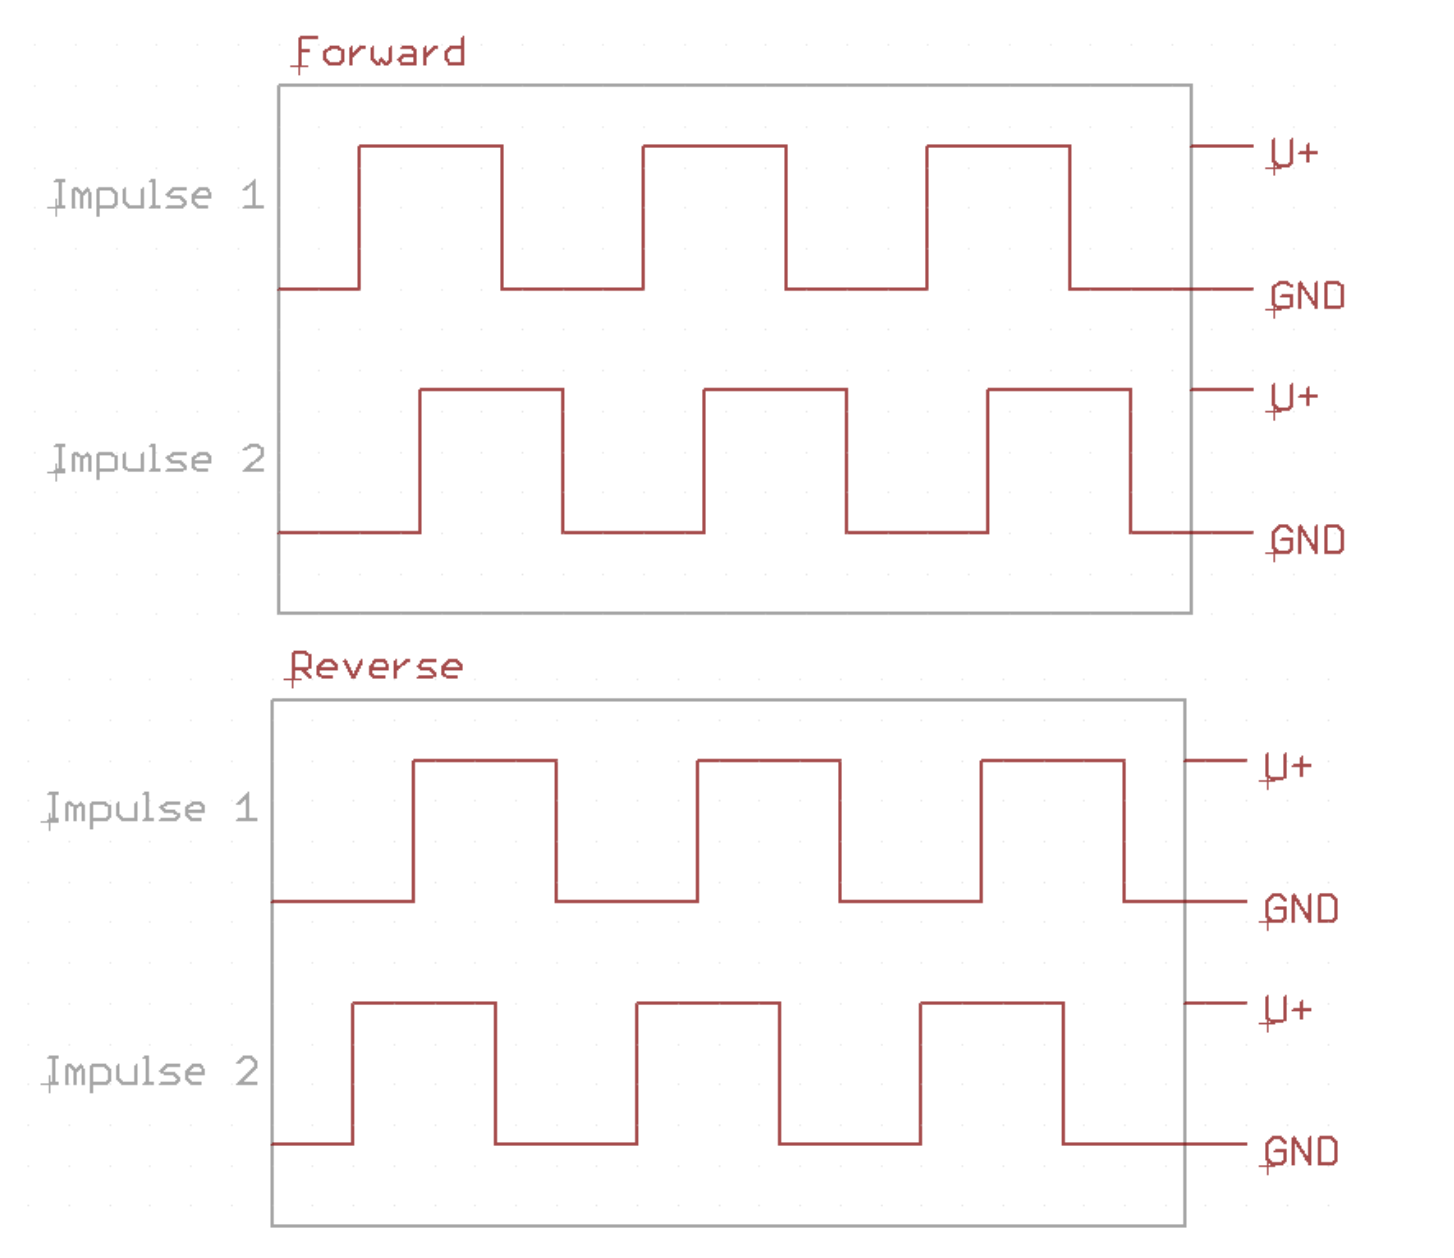
\includegraphics[width=0.8\linewidth]{capitolo2/figure/encoder_signals.png}
\caption{Encoder signals}
\label{fig:encoder_signals}
\end{center}
\end{figure}

The direction of the movement/rotation can be understood by the time order of the two signals generated by the encoder (Figure\ref{fig:encoder_signals}).

\subsection{Push-buttons}
In this project, three LM2T metal push-buttons with spring return produced by Lovato Electronics are used:
\begin{itemize}
    \item a black one (8 LM2T B102) with a normally open contact element is used for the reset operation that moves the robot to the initial position;
    \item a black one (8 LM2T B102) with a normally open contact element is used to start the TCP connection between the PLC and MATLAB;
    \item a red one (8 LM2T B104) with a normally closed contact element is used as a stop emergency button to stop the robot immediately.
\end{itemize}
\begin{figure*}[!h]
\centering
\subfloat[Push-button\label{fig:pushbutton}]{
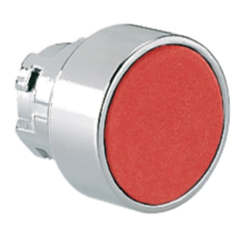
\includegraphics[width=0.25\linewidth]{capitolo2/figure/Push_button.png}
}
\qquad
\subfloat[Normally open contact element\label{fig:no}]{
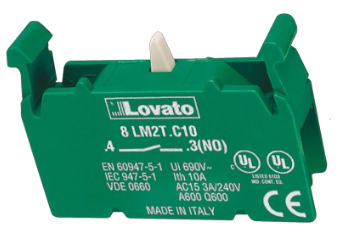
\includegraphics[width=0.25\linewidth]{capitolo2/figure/Normal_open.png}
}
\qquad
\subfloat[Normally closed contact element\label{fig:nc}]{
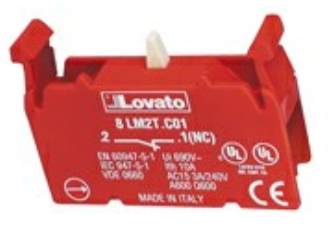
\includegraphics[width=0.25\linewidth]{capitolo2/figure/Normal_closed.png}
}
\caption{Push-buttons}
\label{fig:pushbuttons}
\end{figure*}

\subsection{Light Emitting Diodes}
Two Light Emitting Diodes produced by Lovato Electronics are used in this project. Each LED is made of a LED integrated lamp-holder, a mounting adapter and a pilot light head.
A green LED is turned on when the robot is ready to move and it blinks while the robot is moving.
A red LED is turned on after the emergency stop button has been pressed and it blinks during the reset operation.
\begin{figure*}[!h]
\centering
\subfloat[Light integrated lamp-holder\label{fig:led_integrated}]{
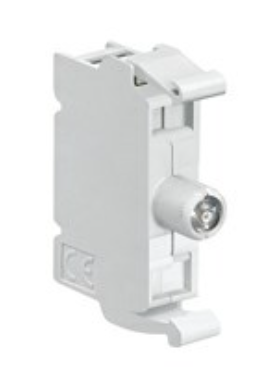
\includegraphics[width=0.25\linewidth]{capitolo2/figure/LED.png}
}
\qquad
\subfloat[Mounting adapter\label{fig:mounting_adapter}]{
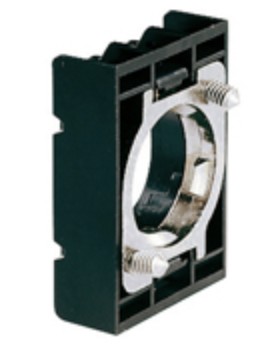
\includegraphics[width=0.25\linewidth]{capitolo2/figure/Mounting_adapter.png}
}
\qquad
\subfloat[Pilot light head\label{fig:light_head}]{
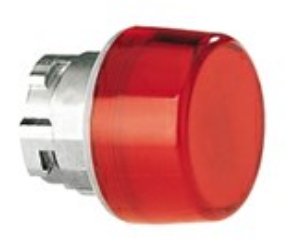
\includegraphics[width=0.25\linewidth]{capitolo2/figure/Light_head.png}
}
\caption{LED}
\label{fig:led}
\end{figure*}

\section{Software}

\subsection{TIA Portal}
TIA Portal (Totally Integrated Automation Portal) is a software package by Siemens created specifically to develop automation using Siemens products such as PLCs. It is in practice a centralized design environment characterized by a common user interface for all automation tasks with shared services (such as those of configuration, communication and diagnostics) and a single database to which also other software packages, such as SIMATIC WinCC V12, SINAMICS Startdrive V12 and SIMATIC STEP 7 PLCSIM V12, access.
The version 15 of the software was used in this project in order to design and upload the control program in the PLC.
TIA Portal has a user interface characterized by the presence of two views:
\begin{itemize}
    \item the portal view;
    \item the project view.
\end{itemize}

\begin{figure*}[!h]
\centering
\subfloat[Portal view\label{fig:portal_view}]{
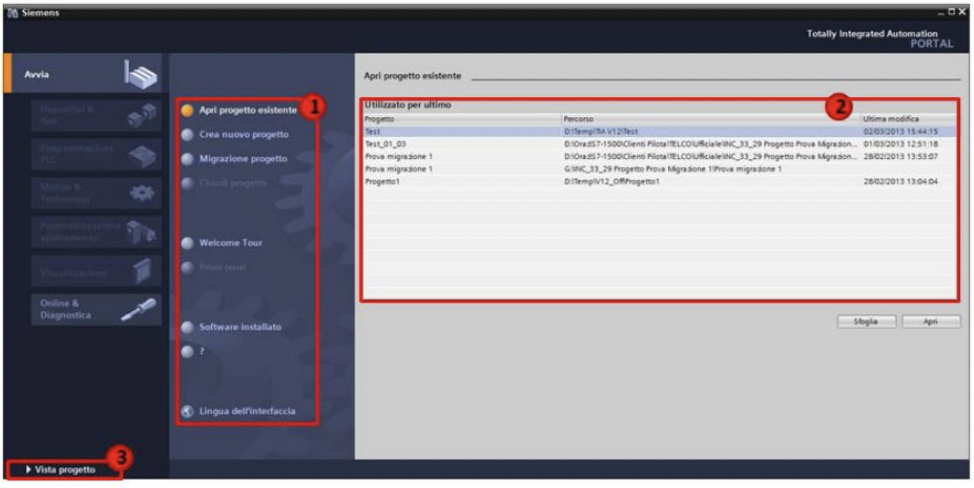
\includegraphics[width=0.45\linewidth]{capitolo2/figure/portal_view.png}
}
\qquad
\subfloat[Project view\label{fig:project_view}]{
\includegraphics[width=0.45\linewidth]{capitolo2/figure/project_view.png}
}
\caption{TIA Portal}
\label{first_signal}
\end{figure*}

\subsubsection{Portal view}
The portal view is the one that opens automatically when it is launched the TIA Portal and that allows the user to choose which operations he wants to perform with the TIA Portal. It is characterized by the presence of:
\begin{enumerate}
    \item a window where it is possible to choose which operation you want to perform;
    \item a selection window related to the selected operation;
    \item a button that allows to switch to the project view.
\end{enumerate}

\subsubsection{Project view}
The project view is the working window of the TIA portal that allows the performance of any function within a project; from the project view it is possible to access all the components of the project and quickly navigate within it.
It is characterized by the presence of:
\begin{enumerate}
    \item a window where it is possible to access and navigate all the components of the project;
    \item a window where the content of the component selected in window 1 is visualized;
    \item a window that allows the user to make changes to the project: the editors for writing of the software, the definition of the hardware or the definition of the panel pages based on the context in which the user is located are displayed;
    \item a window where it is possible to view the properties and the details of the objects selected in the window 3;
    \item a window that varies according to the editor that comes presented in window 3 and allows to view and use the TIA Portal Libraries tool.
\end{enumerate}


%\begin{figure}[!h]
%\begin{center}
%\includegraphics[width=0.8\linewidth]{figure/project_view.png}
%\caption{TIA Portal project view}
%\end{center}
%\label{fig:layout}
%\end{figure}  



%
%\begin{figure*}[!h]
%\centering
%\subfloat[First input signal\label{fig:first}]{%
%\includegraphics[width=0.45\linewidth]{capitolo2/figure/firstinp%ut_out.PNG}%
%}
%\qquad
%\subfloat[First input signal outlier\label{fig:first_det}]{%
%\includegraphics[width=0.45\linewidth]{capitolo2/figure/firstinp%ut_out_detail.PNG}%
%}
%\caption{Plot of the first input signal}
%\label{first_signal}
%\end{figure*}

\subsection{MATLAB}
MATLAB (an abbreviation of "matrix laboratory") is a programming and numeric computing platform developed by MathWorks. MATLAB allows matrix manipulations, plotting of functions and data, implementation of algorithms, data analysis, creation of user interfaces, and interfacing with programs written in other languages.
After starting MATLAB, the desktop appears in its default layout.
\begin{figure}[!h]
\begin{center}
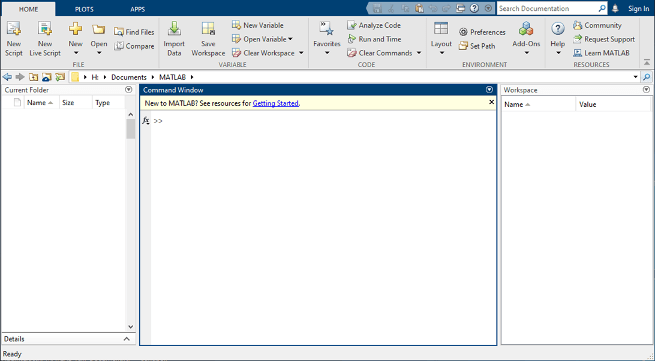
\includegraphics[width=0.6\linewidth]{capitolo2/figure/matlab_desktop.png}
\caption{Matlab desktop}
\end{center}
\label{fig:matlab_desktop}
\end{figure}


The desktop includes these panels:
\begin{itemize}
    \item Current Folder — for file access
    \item Command Window — for entering commands at the command line, indicated by the prompt (>>)
    \item Workspace — for exploring data created or imported from files. \cite{MATLABDo23:online}
\end{itemize} 
%source: matlab documentation
%verify version
In this project a TCP communication between MATLAB (R2021a) and TIA Portal is established to send and receive data continuously. 

\subsection{CoppeliaSim}
CoppeliaSim, formerly known as V-REP (Virtual Robot Experimentation Platform), is a general purpose robot simulator, with integrated development environment, used in industry, education and research for fast algorithm development, factory automation simulations, fast prototyping and verification, robotics related education, motion planning, remote monitoring and safety double-checking. 
CoppeliaSim is based on a distributed control architecture: each object/model can be individually controlled via an embedded script, a plugin, a ROS or BlueZero node, a remote API client, or a custom solution. This makes CoppeliaSim very versatile and ideal for multi-robot applications. Controllers can be written in C/C++ (plug-ins), Lua (scripts acting as individual synchronous controllers), Python, Java,  Matlab or Octave (asynchronous controllers). \cite{Robotsim90:online}
% reference: https://www.coppeliarobotics.com/
% wikipedia:
At its core, CoppeliaSim uses a kinematics engine for forward and inverse kinematics calculations, and several physics simulation libraries to perform rigid body simulation. Models and scenes are built by assembling various objects (meshes, joints, various sensors, Point clouds, OC trees, etc.) into a hierarchial structure. Additional functionality, provided by plug-ins, include: motion planning (via OMPL), synthetic vision and imaging processing (e.g. via OpenCV), collision detection, minimum distance calculation, custom graphical user interfaces and Data visualization (e.g. via plots). \cite{Coppelia94:online}


Scene objects are basic building blocks that can be combined with each other. They can form complex systems together with calculation modules and control mechanisms.

There are fourteen types of scene objects: proximity sensors, graphs, vision sensors, paths, mills, cameras, lights, mirrors, shapes, joints, force / torque sensors, dummies, octrees and point clouds.

There are five calculation modules:
\begin{itemize}
    \item Collision detection
    \item Physics / Dynamics
    \item Minimum distance calculation
    \item Path / Motion planning
    \item Forward / Inverse kinematics
\end{itemize}
%Control mechanisms
%6 methods or interfaces
%>7 languages
%6 methods can be used at the same
%time, and even work hand in hand




 
